


	
	
	%	\hspace{2cm}
	
	\begin{center}
		
\includegraphics[width=0.2\linewidth, height=0.2\textheight]{Upto}
	\end{center}
	
	
	\begin{center}
		{\ {\bf \vspace{0.1cm}  UNIVERSIDAD POLITECNICA \\	TERRITORIAL DEL OESTE\\
				\vspace{0.1cm} 	DE SUCRE\\
		}}
	\end{center}
	
	
	\vskip 0.5cm \rule{\linewidth}{2.3pt}\\[0.5cm]
	\begin{center}
		{\  \LARGE  {\bf \vspace{0.2cm} Introducción al\\				 
				\vspace{0.2cm} Aprendizaje Automático con  Python}} \\ 		
	\end{center}
	
	\vskip 0.5cm \rule{\linewidth}{1.8pt}\\[0.5cm]  
	
	{\bf {\vspace{-1cm} Una Guía para Científicos de Datos}}
	
	
	
	
	\vspace{2cm} 
	\begin{center}
		{\ {\bf \vspace{0.2cm}  	Autor: Andreas C. Müller \& Sarah Guido.\\
				                    Traducido: Prof. Linis B. Guerrero P.\\
				\vspace{0.2cm} 	
		}}
	\end{center}
	
	
	\begin{center}
		{\ {\bf \vspace{0.2cm}  	Cumaná, Venezuela \\
				Octubre, 2019 \\
				\vspace{0.2cm} 
		}}
	\end{center}
	
	
	
	
	
	
	
	
	
	
	\thispagestyle{empty}~~\vspace{-0.2cm}
	
	
	
	%%%%%%%%%%%%%%%%%%%%%%%%%%%%%%%%%%%%%%%%%%%%%%%%%%%%%%%%%%%%%%%%%%%%%%%%%%%%%%%%%%%%%%%%%%%%%% 
	%%%%%%                        Va Una Pagina                                                    %%
	%%%%%%%%%%%%%%%%%%%%%%%%%%%%%%%%%%%%%%%%%%%%%%%%%%%%%%%%%%%%%%%%%%%%%%%%%%%%%%%%%%%%%%%%%%%%%%
	
	
	
	
	
	
	
	
	
	
	
	\begin{center}
		
\includegraphics[width=0.2\linewidth, height=0.2\textheight]{Upto}
	\end{center}
	
	
	\begin{center}
		{\ {\bf \vspace{0.1cm}  UNIVERSIDAD POLITECNICA \\	TERRITORIAL DEL  OCCIDENTE\\
				\vspace{0.1cm} 	DE SUCRE\\
		}}
	\end{center}
	
	
	
	\vskip 0.5cm \rule{\linewidth}{1.3pt}\\[0.5cm]
	\begin{center}
		{\  \LARGE  {\bf \vspace{0.2cm} Introducción al\\				 
				\vspace{0.2cm} Aprendizaje Automático con  Python \\ }}						
	\end{center}		
	
	\vskip 0.5cm \rule{\linewidth}{1.3pt}\\[0.5cm]         
	
	{\bf {\vspace{-0.9cm} Una Guía para Científicos de Datos}}
	
	
	
	
	
	
	\vspace{2cm} 
	
	\begin{center}
		{\ {\bf \vspace{0.2cm}  Trabajo presentado por el Profesor Linis B. Guerrero P.\\ 
				\vspace{0.2cm} 	
		}}
	\end{center}
	
	
	
	
	\begin{center}
		{\ {\bf \vspace{0.2cm}  		Autor: Andreas C. Müller \& Sarah Guido.\\
			                            Traducido: Prof. Linis B. Guerrero P.\\
				\vspace{0.2cm} 	
		}}
	\end{center}
	
	
	\begin{center}
		{\ {\bf \vspace{0.2cm}  	Cumaná, Venezuela \\
				Octubre, 2020 \\
				\vspace{0.2cm} 
		}}
	\end{center}
	
	
	
	
	
	
	
	\thispagestyle{empty}~~\vspace{-0.2cm}
	
	
	
	
	
	
	%%%%%%%%%%%%%%%%%%%%%%%%%%%%%%%%%%%%%%%%%%%%%%%%%%%%%%%%%%%%%%%%%%%%%%%%%%%%%%%%%%%%%%%%%%%%%% 
	%%%%%%                       Van Dos Pagina Universidad                                       %%
	%%%%%%%%%%%%%%%%%%%%%%%%%%%%%%%%%%%%%%%%%%%%%%%%%%%%%%%%%%%%%%%%%%%%%%%%%%%%%%%%%%%%%%%%%%%%%%
	
	
	
	
	% 	\hspace{2cm}
	
	\vskip 5cm \rule{\linewidth}{1.3pt}\\[0.5cm]
	\begin{center}
		{\  \LARGE  {\bf \vspace{0.2cm} Introducción al\\				 
				\vspace{0.2cm} Aprendizaje Automático con  Python \\ }}						
	\end{center}		
	
	\vskip 0.5cm \rule{\linewidth}{1.3pt}\\[0.5cm]         
	
	{\bf {\vspace{-0.9cm} Una Guía para Científicos de Datos}}
	
	
	\thispagestyle{empty}~~\vspace{-0.2cm}
	
	
	%	\vspace{10cm}
	
	\newpage
	
	
	
	
	
	\pagenumbering{Roman}
	\setcounter{page}{1}
	\pagestyle{plain}
	
	
	
	
	
	\chapter*{Agradecimientos} 
	
	
	
	
	
	
	
	
	%	\newpage
	
	\addtocontents{toc}{\hfill \textbf{} \par}
	
	\addtocontents{toc}{\hspace{-7.5mm} \textbf{Capítulos}}
	
	\addtocontents{toc}{\hfill \textbf{Página} \par}
	\addtocontents{toc}{\vspace{-2mm} \hspace{-7.5mm} \hrule \par}
	\addcontentsline{toc}{chapter}{Agradecimientos }	
	
	
	
	\thispagestyle{empty}~~\vspace{-0.2cm}
	
	
	
	
	
	
	\pagenumbering{Roman}
	\setcounter{page}{1}
	\pagestyle{plain}
	
	
	
	
	\thispagestyle{empty}~~\vspace{-0.2cm}
	
	
	\newpage		
	
	\tableofcontents
	\addcontentsline{toc}{chapter}{Índice general }	
	\newpage
	
	\listoffigures
	\addcontentsline{toc}{chapter}{Índice de figuras}	
	\newpage
	
	%	\tablename
    \listoftables
	\addcontentsline{toc}{chapter}{Índice de tablas}	
	\newpage
	
	
	
	
	
	
	
	\chapter*{Prefacio}	
	\addcontentsline{toc}{chapter}{Prefacio}



El aprendizaje automático es una parte integral de muchas aplicaciones comerciales y proyectos de investigación en la actualidad, en áreas que van desde el diagnóstico y tratamiento médico hasta encontrar a tus amigos en las redes sociales. Muchas personas piensan que el aprendizaje automático sólo puede ser aplicado por grandes empresas con amplios equipos de investigación. En este libro, queremos mostrarle lo fácil que puede ser construir soluciones de aprendizaje automático, y cómo hacerlo mejor. Con el conocimiento de este libro, usted puede construir su propio sistema para investigar cómo se siente la gente en Twitter, o hacer predicciones sobre el calentamiento global. Las aplicaciones del aprendizaje automático son infinitas,  y  con la cantidad de datos disponibles hoy en día, en su mayoría limitados por su imaginación.




\section*{Quién debería leer este libro}
\addcontentsline{toc}{section}{Quién debería leer este libro}

Este libro está dirigido a los actuales y futuros profesionales del aprendizaje automático que buscan
implementar soluciones para problemas de aprendizaje automático del mundo real.
Este es un libro introductorio que no requiere conocimientos previos de aprendizaje automático o inteligencia artificial (IA). Nos centramos en el uso de Python y la librería {\ttfamily scikit-learn}, y trabajamos a través de todos los pasos para crear una aplicación de aprendizaje automático exitosa. Las metodologías que presentamos serán útiles para científicos e investigadores, así como para científicos de datos que trabajan en aplicaciones comerciales. Obtendrás el máximo provecho del libro si estás algo familiarizado con Python y las librerías {\ttfamily  NumPy} y  {\ttfamily matplotlib}.\\



Hicimos un esfuerzo consciente para no enfocarnos demasiado en las matemáticas, sino en los aspectos prácticos del uso de algoritmos de aprendizaje automático. Como las matemáticas (teoría de la probabilidad, en particular) es la base sobre la que se construye el aprendizaje automático, no entraremos en el análisis de los algoritmos en gran detalle. Si usted está interesado en las matemáticas de algoritmos de aprendizaje automático, recomendamos el libro The Elements of Statistical Learning (Springer) de Trevor Hastie, Robert Tibshirani, y Jerome Friedman, que está disponible de forma gratuita en el   \href{https://web.stanford.edu/~hastie/ElemStatLearn//}{\color{vino}  sitio web de los autores}. Tampoco describiremos cómo escribir algoritmos de aprendizaje automático desde cero, y en su lugar nos 
centraremos en  cómo utilizar la gran variedad de modelos ya implementados en {\ttfamily scikit-learn} y otras libretías. 

\section*{Por qué escribimos este libro}
\addcontentsline{toc}{section}{Por qué escribimos este libro}

Hay muchos libros sobre aprendizaje automático e inteligencia artificial.
Sin embargo, todos ellos están destinados a estudiantes de posgrado o doctorandos en ciencias de la computación, y con altos contenidos   de matemáticas avanzadas. Esto contrasta marcadamente con la forma en que se utiliza el aprendizaje automático, como una herramienta básica en la investigación y las aplicaciones comerciales. Hoy en día, la aplicación de aprendizaje automático no requiere un doctorado. Sin embargo, hay pocos recursos  que cubran completamente todos los aspectos importantes de la implementación de aprendizaje automático en la práctica, sin necesidad de tomar cursos avanzados de matemáticas. Esperamos que este libro ayude a las personas que quieren aplicar el aprendizaje automático sin tener que  leer o conocer bien el  cálculo, álgebra lineal y teoría de Probabilidad.



\section*{Navegando en este libro}
\addcontentsline{toc}{section}{Navegando en este libro}


Este libro está organizado aproximadamente de la siguiente manera: 

\begin{list}{$\bullet$}{}  
	
	\item  \hyperlink{Cap1}{\color{vino} Capítulo 1} introduce los conceptos fundamentales del aprendizaje automático y sus aplicaciones, y describe la configuración que utilizaremos a lo largo del libro. 
	
	\item En los Capítulos  \hyperlink{Cap2}{\color{vino}2} y \hyperlink{Cap2}{\color{vino}3} se describen los algoritmos reales de aprendizaje automático que se utilizan   ampliamente en la práctica, y se discuten las  ventajas y deficiencias. 
	
	\item En el \hyperlink{Cap4}{\color{vino}Capítulo 4}   discute la importancia de la representación de la data  procesada por  el aprendizaje automático, y a qué aspectos de la data debe prestarle mayor  atención.
	
	\item  El \hyperlink{Cap5}{\color{vino}Capítulo 5}  abarca métodos avanzados de evaluación de modelos y ajuste de parámetros, con especial atención en la validación cruzada y la búsqueda en cuadrícula.
	
	\item  El \hyperlink{Cap6}{\color{vino}Capítulo 6} explica el concepto de {\ttfamily pipelines} para encadenar modelos y encapsular su flujo de trabajo. 
	
	\item  El \hyperlink{Cap7}{\color{vino}Capítulo 7} muestra cómo aplicar los métodos descritos en capítulos anteriores a los datos de texto, e introduce algunas técnicas de procesamiento específicas de texto. 
	
	\item  El \hyperlink{Cap8}{\color{vino}Capítulo 8}  ofrece una visión general de alto nivel e incluye referencias a temas más avanzados.
	
\end{list}


Mientras que los capítulos 2 y 3 proporcionan  algoritmos reales, entender todos estos algoritmos podría no ser necesario para un principiante. Si necesita construir un sistema de aprendizaje automático lo antes posible, le sugerimos comenzar con el capítulo 1 y las secciones iniciales del capítulo 2, que introducen todos los conceptos básicos. A continuación, puede saltar a "{}Resumen y Outlook"{} en la página \pageref{Pagina127} en el capítulo \ref{Cap2}, que incluye una lista de todos los modelos supervisados que cubrimos. Elige el modelo que mejor se adapte sección dedicada a ella para los detalles. A continuación, puede utilizar las técnicas del capítulo 5 para evaluar y afinar su modelo.


Elija el modelo que mejor se adapte a sus necesidades y vuelva atrás para leer la sección dedicada al modelo para  más detalles.   Puede utilizar las técnicas del Capítulo \ref{Cap5} para evaluar
y ajustar el modelo seleccionado.


\section*{Recursos en línea}
\addcontentsline{toc}{section}{Recursos en línea}

Al estudiar este libro, puede visitar el sitio web {\ttfamily scikit-learn}   para obtener documentación detallada sobre  clases, funciones, y muchos ejemplos. También hay un curso con  vídeos creado por Andreas Müller,  "{}Aprendizaje Automático Avanzado con scikitlearn"{}, que complementa este libro. Puede encontrarlo en  \href{https://www.oreilly.com/library/view/advanced-machine-learning/9781771374927/}{\color{vino}   http://bit.ly/advanced\_machine\_learning\_scikit-learn}.


\section*{Convenciones utilizadas en este libro}
\addcontentsline{toc}{section}{Convenciones utilizadas en este libro}


En este libro se utilizan las siguientes convenciones tipográficas:\\

\noindent{\bf{Italic}}

\noindent Indica nuevos términos, direcciones URL, direcciones de correo electrónico, nombres de archivo y extensiones de archivo. \\

\noindent {\bf{Constant width}}

\noindent Usado para listados de programas, así como dentro de párrafos para referirse a elementos de programas tales como nombres de variables o funciones, bases de datos, tipos de datos, variables de entorno, sentencias y palabras clave. También se utiliza para comandos y nombres de módulos y paquetes. \\


\noindent {\bf Constant width bold}

\noindent Muestra comandos u otro texto que el usuario debe escribir literalmente.\\ 


\noindent {\bf Constant width italic}

\noindent Muestra texto que debe reemplazarse por valores proporcionados por el usuario o por valores determinados por el contexto. \\


\vspace{0.3cm}
\noindent \begin{minipage}[t]{0.2\textwidth}
	\centering\raisebox{\dimexpr \topskip-\height}{%
		
\includegraphics[scale=0.35]{Imagen_Machine/Zorrillo.png}}
\end{minipage}%\hfill
\begin{minipage}[t]{0.75\textwidth} 
	
	Este elemento significa una sugerencia o sugerencia.
\end{minipage}
\vspace{0.3cm}



\vspace{0.2cm}
\noindent \begin{minipage}[t]{0.2\textwidth}
	\centering\raisebox{\dimexpr\topskip-\height}{%
		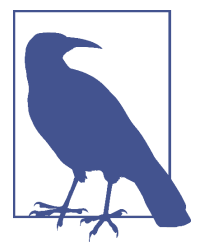
\includegraphics[scale=0.35]{Imagen_Machine/Pajaro.png}}  %[width=\textwidth]
	
\end{minipage}%\hfill
\begin{minipage}[t]{0.75\textwidth} 
	
	Este elemento significa una nota general.
\end{minipage}
\vspace{0.2cm}



\vspace{0.3cm}
\noindent\begin{minipage}[t]{0.2\textwidth}
	\centering\raisebox{\dimexpr \topskip-\height}{%
		
\includegraphics[scale=0.35]{Imagen_Machine/Escorpion}}  
\end{minipage}%\hfill
\begin{minipage}[t]{0.70\textwidth} 
	
	Este icono indica una advertencia o precaución.
\end{minipage} 
\vspace{0.5cm}

\section*{Uso de ejemplos de código}
\addcontentsline{toc}{section}{Uso de ejemplos de código}


El  material suplementario (ejemplos de código, cuadernos IPython, etc.) está disponible para su descarga en:


\hspace{0.5cm} \href{https://github.com/amueller/introduction_to_ml_with_python}{\color{vino} https://github.com/amueller/introduction\_to\_ml\_with\_python}.\\

Este libro se desarrolló con la finalidad de  ayudarle en  su trabajo. En general, el  código en los  ejemplo del libro lo puede usar en sus programas y documentación. No necesita contactar con nosotros para obtener permiso a menos que esté reproduciendo una parte significativa del código. Por ejemplo, escribir un programa que usa varios trozos de código de este libro no requiere permiso. Vender o distribuir un CD-ROM de ejemplos de libros de O'Reilly requiere permiso. Responder a una pregunta citando este libro y citando el código de ejemplo no requiere permiso. La incorporación de una cantidad significativa de código de ejemplo de este libro en la documentación de su producto requieren permiso.\\



Agradecemos la atribución, pero no la exigimos.  Una atribución generalmente incluye el título, autor, 
editor e ISBN. Por ejemplo: {\emph{"{}Una introducción al aprendizaje automático con Python}} por 
Andreas C. Müller y Sarah Guido (O'Reilly). Copyright 2017 Sarah Guido y Andreas Müller, 978-1-449-36941-5."{} \\


Si cree que el uso que hace de los ejemplos de código queda fuera del uso legítimo o del permiso otorgado
arriba, no dude en contactarnos en {\color{vino} permissions@oreilly.com}. 

\section*{Libros online Safari}
\addcontentsline{toc}{section}{Libros online Safari}

\noindent Safari\textsuperscript{\textbf{\tiny\textregistered}} Books Online\\
%  \noindent Safari$^{{\bf\tiny®}}$ Books Online\\   Error cambiar $^ por \textsuperscript{ }

\vspace{0.3cm}
\noindent\begin{minipage}[t]{0.2\textwidth}
	\centering\raisebox{\dimexpr \topskip-\height}{%
		
\includegraphics[scale=0.25]{Imagen_Machine/Safari}}  
\end{minipage}%\hfill
\begin{minipage}[t]{0.8\textwidth} 
	\href{http://safaribooksonline.com/}{\color{vino} Safari Books Online} es una librería  digital bajo demanda que ofrece contenido experto en forma de libro y vídeo de los principales autores mundiales en tecnología y negocios.
\end{minipage} 
\vspace{0.5cm}


%   Safari$^{{\bf\tiny ®}}$ Books Online\\



Los profesionales de la tecnología, los desarrolladores de software, los diseñadores web, y los profesionales comerciales y creativos utilizan Safari Books Online como su principal recurso para la investigación, resolución de problemas, aprendizaje, entrenamiento y  la certificación.\\



Safari Books Online ofrece una gama de  \href{https://www.safaribooksonline.com/pricing/}{\color{vino} planes y precios}  para  \href{https://www.safaribooksonline.com/enterprise/}{\color{vino} empresas},  
\href{https://www.safaribooksonline.com/government/}{\color{vino} gobiernos},  \href{https://www.safaribooksonline.com/academic-public-library/ }{\color{vino} educación}  y personales o individuales.\\


Los miembros tienen acceso a miles de libros, videos de capacitación y manuscritos de prepublicación en una base de datos de búsqueda completa de editores como   O’Reilly Media, Prentice Hall Professional, Addison-Wesley Professional, Microsoft Press, Sams, Que, Peachpit Press, Focal Press, Cisco Press, John Wiley \& Sons, Syngress, Morgan Kaufmann, IBM Redbooks, Packt, Adobe Press, FT Press, Apress, Manning, New Riders,
McGraw-Hill, Jones \& Bartlett, Course Technology,  y \href{https://www.oreilly.com/our-library/}{\color{vino} centenares más}. Para más información acerca de Libros de Safari Online, por favor visita nuestra  \href{https://www.oreilly.com/}{\color{vino} online}.\\




Safariķ Books Online Safari Books Online es una biblioteca digital bajo demanda que ofrece contenido experto en forma de libro y vídeo de los principales autores mundiales en tecnología y negocios.


%   http://safaribooksonline.com/




\section*{Como contactar con nosotros}
\addcontentsline{toc}{section}{Como contactar con nosotros}


Dirija sus comentarios y preguntas sobre el libro al editor:\\


O’Reilly Media, Inc.

1005 Gravenstein Highway North

Sebastopol, CA 95472

800-998-9938 (in the United States or Canada)

707-829-0515 (international or local)

707-829-0104 (fax)\\




Tenemos una página web para este libro, con la fe de erratas, ejemplos y cualquier información adicional. Puede acceder a esta página en:\\ \href{http://bit.ly/intro-machine-learning-python}{\color{vino}http://bit.ly/intro-machine-learning-python}.\\

Para comentar o hacer preguntas técnicas sobre este libro, envíe un correo electrónico a {\color{vino} bookquestions@oreilly.com}.\\

Para obtener más información sobre nuestros libros, cursos, conferencias y noticias, consulte nuestro sitio web en \href{https://www.oreilly.com/}{\color{vino} http://www.oreilly.com}.\\

Encuéntrenos en Facebook:   \href{ http://facebook.com/oreilly}{\color{vino} http://facebook.com/oreilly}.\\
Síganos en Twitter:   \href{ http://twitter.com/oreillymedia}{\color{vino} http://twitter.com/oreillymedia}.\\
Míranos en YouTube:   \hspace{0.5cm} \href{http://www.youtube.com/oreillymedia}{\color{vino} http://www.youtube.com/oreillymedia}.\\


\section*{Agradecimientos}
\addcontentsline{toc}{section}{Agradecimientos}

{\bf{De Andreas}}


Sin la ayuda y el apoyo de un gran grupo de personas, este libro nunca habría existido.\\

Me gustaría agradecer a los editores, Meghan Blanchette, Brian MacDonald, y en particular a Dawn Schanafelt, por ayudarnos tanto a Sarah y como a  mí,  a hacer de este libro una realidad.\\

Quiero agradecer a mis críticos, Thomas Caswell, Olivier Grisel, Stefan van der Walt, y John Myles White, que se tomó el tiempo de leer las primeras versiones de este libro y me proporcionó una valiosa retroalimentación, además de ser algunas de las piedras angulares del ecosistema científico 
de código abierto.\\


Estoy eternamente agradecido por la acogedora comunidad científica de código abierto de Python, 
especialmente los contribuyentes a {\ttfamily scikit-learn}. Sin el apoyo y la ayuda de esta comunidad, 
en particular de Gael Varoquaux, Alex Gramfort, y Olivier Grisel, nunca me habría convertido en un contribuyente principal a {\ttfamily scikit-learn} o aprender a entender  este paquete tan bien como lo hago ahora.   Mi agradecimiento también va a todos los otros contributores que donan su tiempo para mejorar y 
mantener este paquete.\\ 


También estoy agradecido por las discusiones con muchos de mis colegas y compañeros que me ayudaron
a comprender los desafíos del aprendizaje automático y me dio ideas para la estructura un libro de texto. Entre las personas con las que hablo sobre el aprendizaje automático, específicamente quiero agradecer a Brian McFee, Daniela Huttenkoppen, Joel Nothman, Gilles Louppe, Hugo Bowne-Anderson, Sven Kreis, Alice Zheng, Kyunghyun Cho, Pablo Baberas, y Dan Cervone.\\



Mi agradecimiento también va para Rachel Rakov, quien fue una ansiosa beta tester y correctora
de una de las primeras versiones de este libro y me ayudó a darle forma de muchas maneras.\\


En el aspecto personal, quiero agradecer a mis padres, Harald y Margot, y a mi hermana,
Miriam, por su continuo apoyo y aliento. También quiero agradecer a muchas personas en mi 
vida cuyo amor y amistad me dieron la energía y el apoyo para emprender una tarea tan desafiante.\\



{\bf{De Sarah}}


Me gustaría agradecer a Meg Blanchette, sin cuya ayuda y orientación este proyecto
ni siquiera habría existido. Gracias a Celia La y Brian Carlson por leerlo en los primeros días. Gracias a la gente de O'Reilly por su infinita paciencia. Y finalmente gracias a DTS, por su apoyo eterno e infinito.



	
	
	
	
	
%	\addcontentsline{toc}{chapter}{Resumen }	
	
	\newpage
	
	\pagenumbering{arabic}
	\setcounter{page}{1}
	\pagestyle{plain}
	
	
	
	
	
	
	
	\addcontentsline{toc}{chapter}{Prefacio}
	
	
	\setcounter{secnumdepth}{3}
	
	
	
	\setcounter{tocdepth}{3}
	
	
	
	
	
	
